\documentclass{scrartcl}
\usepackage{notes}
\usepackage[numbers]{natbib}
\usepackage{cleveref}


\title{(Continuous) Normalizing Flows}
\setheader{(Continuous) Normalizing Flows}
\date{November, 2025}

\begin{document}

\maketitle


\section{Generative Modeling}
\todo{Add in discussion about how we can generally interact with the target distribution by sampling, so that any objective function should ideally be formulated as an expectation with resect to the true distribution.}
The premise of modern generative modeling, at least in the context of machine learning, is that the task of \textit{generation} can be framed as one of \textit{sampling} from the appropriate probability distribution $p(x)$. For example, the generation of a 28 by 28 RGB image can be modeled as sampling from a hypothetical distribution $p_{\textit{image}}(x) \in \mathcal{P}(\mathbb{R}^{28\times28\times3})$.

\begin{problembox}
How do we actually sample from  $p_{\textit{image}}(x)$?
\end{problembox}

The solution is generally to construct, or \textit{learn}, some variational approximation $p(x; \theta) \approx \pdata(x)$. 
Over finite/categorical spaces, this is significantly easier, and one can simply paramterize $p(x; \theta)$ directly as the probability mass within each category. For distributions defined over continuous spaces, this is no longer possible. What then do we do? In these notes, we explore one family of approaches toward learning such a $p_\theta$, namely \textit{normalizing flows}.

\section{Normalizing Flows}
The idea behind normalizing flows, and indeed much of modern flow-based generative modeling is to realize the distribution of interest - $p_{\text{data}}$ - as some learned deformation of a simple distribution $p_0(x)$ that we \textit{can} sample from (usually a Gaussian). We make this precise via the notion of a \textit{pushforward} which we define below.
\begin{defbox}[Pushforward]
    Consider the random variable obtained via the following procedure:
    \begin{itemize}
        \item Sample $x_0 \sim p_0$.
        \item Compute $x_1 \triangleq f(x_0; \theta)$.
    \end{itemize}
    Here, $f$ is some learned, \textit{invertible}, squishing agent. Then $x_1$ is itself a random variable, and has a distribution $p_1(x;\theta)$ which we'll define as the \textit{pushforward} of $p_0$ by $f(\cdot;\theta)$, and which is sometimes denoted as $f(\cdot;\theta)_\sharp p_0$.
\end{defbox}
Now, how would we actually learn $f$? The usual idea is to choose some rich parametric family for $f(\cdot; \theta)$ (usually some sort of neural network; we'll this later), and minimize the Kullback-Leibler (KL) divergence, and find
\begin{align*}
\theta^\ast&\triangleq \argmin_\theta \dkl{\pdata}{p(\cdot; \theta)}\\
&= -\EE_{x \sim \pdata} \left[\log p(x; \theta)\right] - H(\pdata)\\
&= \argmax_{\theta} \EE \left[\log p(x; \theta)\right]
\end{align*}
which yields the usual ``maximum-likelihood" objective. Now, recall from calculus that the density of the pushforward $p_1(x; \theta)$ is then given by the change of variables formula from calculus,
\begin{equation}
p_1(x_1; \theta) = p_0(x_1)\det\abs*{\pdv{f(x_0;\theta)}{x_0}}^{-1},
\end{equation}
or equivalently,
\begin{equation}
    \log p_1(x_1; \theta) = \log p_0(x_1) - \log \det\abs*{\pdv{f(x_0;\theta)}{x_0}}^{-1}
    \label{eq:cov}
\end{equation}
which in particular is a differentiable function of $\theta$. We therefore arrive at the following desiderata:
\begin{itemize}
    \item The function $f_\theta$ should be invertible.
    \item The function should be constructed in such a way that $ \log \det\abs*{\pdv{f(x_0;\theta)}{x_0}}^{-1}$ is cheap to evaluate analytically, or at least to approximate.
\end{itemize}
The general idea in flows is to find a bunch of smaller building blocks $\{f_i(\cdot; \theta)\}$ which satisfy the above two criteria, and then chain them together so as to obtain $f$ as the composition
\begin{equation}
f(x_0; \theta) \triangleq f^N(\cdot; \theta_N) \circ \dots \circ f^1(\cdot; \theta_1).
\end{equation}
Let's take a look at a few examples.
\begin{examplebox}[RealNVP]
The authors of \citep{realnvp} propose to partition $x = \begin{bmatrix}x_1 & x_2\end{bmatrix}$ and construct $f^i$ as a non-volume-preserving shear transformation
\begin{equation}
    \begin{bmatrix} y_1 \\ y_2 \end{bmatrix} = f\left(\begin{bmatrix} x_1 \\ x_2 \end{bmatrix}\right) = \begin{bmatrix} \alpha(x_2; \theta) \odot x_1 + \beta(x_2) \\ x_2 \end{bmatrix}.
\end{equation}
Then it's easy to verify that $f^i$ is invertible and that 
\begin{equation}
\pdv{y}{x} = \begin{bmatrix} \text{diag}(\alpha) & \cdots \\ 0 & I \end{bmatrix}
\end{equation}
from which it immediately follows that $\det\abs*{\pdv{y}{x}} = \prod_i \alpha_i$.
\end{examplebox}

\begin{examplebox}[Autoregressive Flows]
    The previous construction can be generalized to partition size, yielding so-called \textit{autoregressive flows}. Indexing the components of $x$ as $x_i$, the authors of \citep{iaf}
    propose the \textit{inverse autoregressive} flow update
    \begin{equation}
    y_{d} = \alpha(x_{<d};\theta) \odot x_d + \beta(x_{<d}; \theta)
    \end{equation}
    while the authors of \citep{maf} propose the \textit{masked autoregressive} flow update
    \begin{equation}
    y_{d} = \alpha(y_{<d};\theta) \odot x_d + \beta(y_{<d}; \theta).
    \end{equation}
    In each case, we can verify that the proposed transformations are invertible and yield block-diagonal Jacobians with readily available determinant.
\end{examplebox}

\begin{examplebox}[TarFlow]
    It was only a matter of time before somebody added a transformer to the mix, and Apple of all places did just that in December 2024 with the introduction of TarFlow \citep{tarflow}. Recent work has extended TarFlow to the latent space of a learned VAE \citep{starflow} and to molecular conformer generation \citep{amortized_sampling}.
\end{examplebox}

Althoug recent work has made strides toward resolving this (see e.g., \citep{tarflow} and \citep{starflow}), normalizing flows still suffer from restrictive architectural constraints.

\section{Continuous Normalizing Flows}
How might we relax these architectural constraints? Continuous normalizing flows propose to avoid the restrictions placed on $f(\cdot; \theta)$ by instead parameterizing it indirectly as the time-evolution of a learned vector field. 
That is, instead of obtaining $x_1$ directly via an application of a learned $f(\cdot; \theta)$, we will obtain it via the following procedure:
\begin{itemize}
\item Sample $x_0 \sim p_0(x)$.
\item Obtain $x_1$ by solving the initial value problem (IVP) given by our sampled $x_0$ and \begin{equation}
\d x_t = u_t(x; \theta)\, \d t. \label{eq:cnf}
\end{equation}
\end{itemize}
\subsection{Change of Variables in Continuous Time}
We remark that our general normalizing flow recipe is still intact from earlier is still intact, although it remains to get a handle on the log density $\log p_1(x_1; \theta)$. In particular, by switching to parameterizing $f$ via the vector field $u$, we trade harsh invertibility/tractable differentiability constraints for mild regularity constraints (namely Lipschitz continuity, which can be guaranteed for neural networks).

\begin{resultbox}[Continuous change of variables \citep{neural_ode}]
Define $p_t(x_t;\theta)$ as the distribution of $x_t$. Then 
\begin{equation}
\frac{\d}{\d t} \log p_t(x_t;\theta) = - \nabla \cdot u(x_t; \theta),
\end{equation}
where $\nabla$ denotes the divergence.
\end{resultbox}
\begin{proof*}{Proof sketch}
We follow along \citep{neural_ode}. Define $f_{t,s}: x_t \mapsto x_s$ as the ``time-evolution" map from time $t$ to time $s$, for $s > t$, and so that $f = f_{0,1}$. Then, by definition of the derivative
\begin{align*}
    \frac{\d}{\d t} \log p_t(x_t;\theta) &= - \frac{\d}{\d t} \log \det\abs*{\pdv{f_{0,t}}{x_0}}\\
    &= - \frac{1}{\det\abs*{\pdv{f_{0,t}}{x_0}}}\lim_{\varepsilon \to 0} \frac{\det\abs*{\pdv{f_{0,t + \varepsilon}}{x_t}} - \det\abs*{\pdv{f_{0,t}}{x_0}}}{\varepsilon}\\
    &= - \frac{1}{\det\!\left(\pdv{f_{0,t}}{x_t}\right)}
   \lim_{\varepsilon \to 0}
   \det\!\left(\pdv{f_{0,t}}{x_0}\right)
   \left(
      \frac{
        \det\!\left(\pdv{f_{t,t+\varepsilon}}{x_t}\right)
        - \det(I)
      }{\varepsilon}
   \right)\\
   &= -\lim_{\varepsilon \to 0}
      \frac{
        \det\!\left(\pdv{f_{t,t+\varepsilon}}{x_t}\right)
        - \det(I)
      }{\varepsilon}
\end{align*}
Applying L'Hôpital's rule yields
\begin{align*}
    \lim_{\varepsilon \to 0}
    \frac{
      \det\!\left(\pdv{f_{t,t+\varepsilon}}{x_0}\right)
      - \det(I)
    }{\varepsilon} &= -\lim_{\varepsilon \to 0}
    \frac{\d}{\d \varepsilon}
      \det\!\left(\pdv{f_{t,t+\varepsilon}}{x_0}\right)\\
      &= - \lim_{\varepsilon \to 0} \tr(\adj\left(\pdv{f_{t,t+\varepsilon}}{x_t}\right)\frac{\d}{\d \varepsilon}\pdv{f_{t,t+\varepsilon}}{x_0})\\
      &= - \tr\!\left[
        \underbrace{\left(
            \lim_{\varepsilon \to 0}
          \adj\!\left( \pdv{f_{t,t+\varepsilon}}{x_t} \right)
        \right)}_{\to I}
        \left(
            \lim_{\varepsilon \to 0}
          \frac{\d}{\d\varepsilon}\!\left( \pdv{f_{t,t+\varepsilon}}{x_t} \right)
        \right)
    \right]\\
    &= - \tr
        \lim_{\varepsilon \to 0}
        \frac{\partial}{\partial x_t}
        \underbrace{
          \left(
            \frac{\d f_{t,t+\varepsilon}}{\d \varepsilon}
          \right)
        }_{u_{t+\varepsilon}(x_{t+\varepsilon};\theta)}\\
    &= -\tr \left(\frac{\partial u_t}{\partial x_0}\right)\\
    &= - \nabla \cdot u_t(x_t; \theta)
\end{align*}
as claimed. Here, the first equality follows from \href{https://en.wikipedia.org/wiki/Jacobi%27s_formula}{Jacobi's formula}, and where $\adj(A)$ denotes the \textit{adjugate} matrix (transpose of cofactor matrix). Importantly, we used the fact that the adjugate of the identity is the identity.
\end{proof*}

\subsection{Backpropagation in Continuous Time}
Recall that 
\begin{equation}
\begin{aligned}
x_1 &= x_0 + \int_0^1 u_t(x_t;\theta)\, \d t\\
\log p_1(x_1;\theta) &= \log p_0(x_0) - \int_0^1 \nabla \cdot u_t(x_t; \theta)
\end{aligned}
\label{eq:cnf_setup}
\end{equation}
and that our objective remains to obtain
\begin{equation}
    \theta^\ast \triangleq \argmax_{\theta}\EE_{x_1 \sim \pdata} \left[\mathcal{L}(x_1;\theta)\right]\\
    \mathcal{L}(x_1; \theta) \triangleq \log p(x; \theta).
\end{equation}
To this end, we seek an expression for $\nabla_\theta \mathcal{L}(\theta)$. 

\begin{figure}
    \centering
    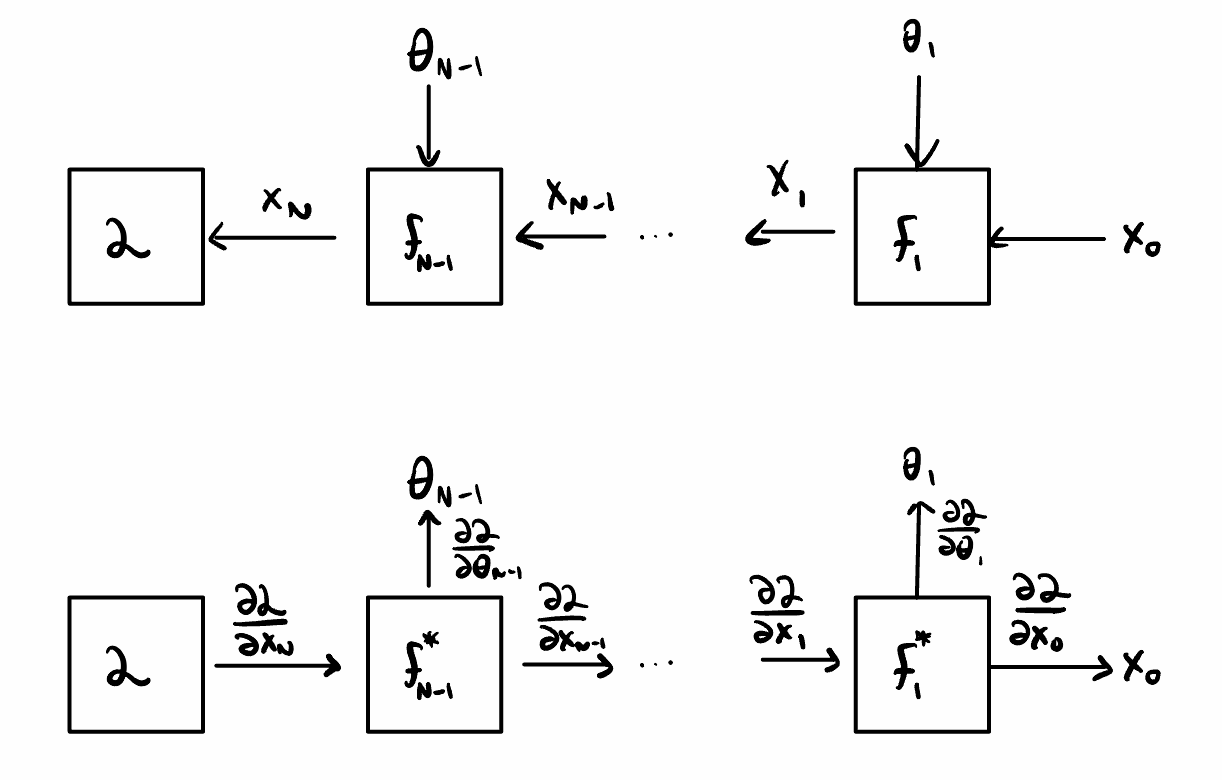
\includegraphics[scale=0.4]{images/backprop.png}
    \caption{Backpropagation through a discrete neural network.}
    \label{fig:backprop}
\end{figure}

\begin{backgroundbox}[Backpropagation]
Recall that traditionally, the gradients of a a loss with respect to a neural network's weights are computed by reveres-mode automatic differentiation, or \textit{backpropagation}. 
    With back propagation, the idea is to traverse the \textit{computation graph} backwards, and use the chain rule to recursively compute the gradients. In the usual case that the reverse-traversal path from any node to a weight passes through some intermediate activation $x_t$, it becomes necessary to compute the \textit{activation gradients} $\frac{\partial \mathcal{L}}{\partial x_t}$ as well. 
    We summarize this procedure in \cref{fig:backprop}
\end{backgroundbox}



The takeaway from \cref{fig:backprop} is that the weight gradients $\frac{\partial \mathcal{L}}{\partial \theta}$ are the \textit{leaves} of the backpropagation graph. 
To compute these, we must simultaneously compute the gradients $\frac{\partial \mathcal{L}}{\partial x_t}$. 
In the discrete setting of \cref{fig:backprop}, the intermediate states $x_t$ are often referred to as \textit{activations}, so that we might refer to $\frac{\partial \mathcal{L}}{\partial x_t}$ as activation gradients. 
In order to get an intuitive sense for what these gradients should be, let's consider a discretization of our continuous normalizing flow, and see about computing the gradients in this slightly similar setting. 
In particular, let $\mathbf{t} \triangleq \{t_i\}_{i=0}^N$ with $0 = t_0 < \cdots < t_N = 1$, and consider 
\begin{equation}
    \begin{aligned}
    x_{t_{i+1}} &= x_{t_i} + u_{t_i}(x_{t_i},t;\theta)\, \Delta t_i\\
    \mathcal{L}(x;\theta) &= \log p_0(x_0) - \sum_{i=0}^N \nabla \cdot u_{t_i}(x_{t_i}; \theta)\, \Delta t_i
    \end{aligned}
    \label{eq:discrete_cnf_setup}
\end{equation}
as a discrete analog of \cref{eq:cnf_setup}. Before we dive in, and to make our task conceptually clearer, observe that sensitivity of $\mathcal{L}$ to a perturbation of $\theta$ (i.e., $\frac{\partial \mathcal{L}}{\partial \theta}$) naturally decomposes into the sum of sensitivities of $\mathcal{L}$ with respect to the perturbations of $\theta$ at each distinct timestep $t_i$. We will therefore adopt the notation $\theta_{t_i}$ to refer to the (uniform) value of $\theta$ at $t_i$, and so that $\pdv{\mathcal{L}}{\theta_{t_i}}$ is understood to denote the sensitivity of $\mathcal{L}$ to $\theta_{t_i}$ if the value of $\theta$ at all other timesteps are held constant.
For brevity, we will henceforth denote by $a^x_{t_i}$ the activation gradient $\frac{\partial \mathcal{L}}{\partial x_{t_i}}$, and by $a^\theta_{t_i}$ the weight gradient $\frac{\partial \mathcal{L}}{\partial \theta_{t_i}}$. Then, it follows immediately from \cref{eq:discrete_cnf_setup} that $a^x_{t_i}$ satisfies the recursion
\begin{equation*}
a^x_{t_i} = \underbrace{a^x_{t_{i+1}} \frac{\partial x_{t_{i+1}}}{\partial x_{t_i}}}_{\text{upstream sensitivity}} - \underbrace{\frac{\partial}{\partial x_{t_i}} \nabla \cdot u_{t_i}(x_{t_i},t;\theta_{t_i}) \Delta t_i}_{\text{direct sensitivity}},
\end{equation*}
which makes precise the observation that perturbing $x_{t_i}$ affects $\mathcal{L}$ \textit{indirectly} by perturbing the values of the downstream $x_{t_{>i}}$, as well as \textit{directly} via the loss contribution in $\nabla \cdot u_{t_i}(x_{t_i},t_i;\theta_{t_i})$. Plugging in $\frac{\partial x_{t_{i+1}}}{\partial x_{t_i}} = I + \Delta t_i  \frac{\partial u_{t_i}}{\partial x_{t_i}}$, and rearranging yields
\begin{equation*}
\frac{a^x_{t_{i+1}} - a^x_{t_{i}}}{\Delta t_i} = -a^x_{t_{i+1}} \frac{\partial u_{t_i}}{\partial x_{t_i}} + \frac{\partial}{\partial x_{t_i}} \nabla \cdot u_{t_i}(x_{t_i},t_i;\theta_{t_i}).
\end{equation*}
Finally, taking $\Delta t_i \to 0$ suggests that in the infinite limit, $a_t^x$ satisfies $\frac{\d}{\d t} a^x_t = -a^x_t \frac{\partial u_t}{\partial x_t} + \frac{\partial}{\partial x_t} \nabla \cdot u_t(x_t,t;\theta_{t_i})$. For $a^\theta_t$, we similarly derive the recurrence
\begin{equation*}
    a^\theta_{t_i} = \underbrace{a^x_{t_{i+1}} \frac{\partial x_{t_{i+1}}}{\partial \theta_{t_i}}}_{\text{upstream sensitivity}} - \underbrace{\frac{\partial}{\partial \theta_{t_i}} \nabla \cdot u_{t_i}(x_{t_i},t;\theta_{t_i}) \Delta t_i}_{\text{direct sensitivity}},
\end{equation*}



\begin{resultbox}[Adjoint state IVP \citep{neural_ode}]
The \textit{adjoint state} \begin{equation} a_t = \begin{bmatrix}a_t^x & a_t^\theta \end{bmatrix}^T \triangleq \begin{bmatrix} \frac{\partial \mathcal{L}(x_t; \theta)}{\partial x_t } \frac{\partial \mathcal{L}(x_t; \theta)}{\partial \theta_t}\end{bmatrix}^T\end{equation} satisfies the IVP
\begin{equation}
\frac{\d}{\d t} \begin{bmatrix}a_t^x \\ a_t^\theta \end{bmatrix} = \begin{bmatrix} 
    -a_t^x\frac{\partial u_t}{\partial x_t} + \frac{\partial}{\partial x_t} \nabla \cdot u_t(x_t; \theta) \\
    -a_t^x \frac{\partial u_t}{\partial \theta} + \frac{\partial}{\partial \theta_t} \nabla \cdot u_t(x_t; \theta).
\end{bmatrix}
\end{equation}
\end{resultbox}

\begin{proof*}{Proof sketch}
    The essential idea is that for any $\varepsilon > 0$ (and sufficiently small), we may obtain the recursion 
    \begin{equation}
        a_t
        = a_{t+\varepsilon}\,
        \frac{
          \partial \begin{bmatrix} x_{t+\varepsilon} & \theta_{t+\varepsilon} \end{bmatrix}
        }{
          \partial \begin{bmatrix} x_t & \theta_t \end{bmatrix}
        }
        \;-\;
        \frac{\partial}{\partial \begin{bmatrix} x_t & \theta_t \end{bmatrix}}
        \int_t^{t+\varepsilon} \nabla \!\cdot u(x_s;\theta)\, \d s.
    \end{equation}
    with
    \begin{align*}
        \frac{\partial \begin{bmatrix} x_{t+\varepsilon} & \theta_{t+\varepsilon} \end{bmatrix}}{\begin{bmatrix} x_t & \theta_t \end{bmatrix}} &= \frac{\partial}{\partial {\begin{bmatrix} x_t & \theta_t \end{bmatrix}}}\begin{bmatrix} x_t \\ \theta_t \end{bmatrix} + \varepsilon\underbrace{\begin{bmatrix} \frac{\partial u_t}{\partial x_t} \\ 0 \end{bmatrix}}_{\frac{\d}{\d \varepsilon} x_{t + \varepsilon}} + \mathcal{O}(\varepsilon^2)\\
        &= I + \varepsilon \begin{bmatrix} \frac{\partial}{\partial x_t} u_t & \frac{\partial}{\partial \theta_t} u_t \\ 0 & 0 \end{bmatrix} + \mathcal{O}(\varepsilon^2).
    \end{align*}
    Plugging the above into the definition of the derivative, we thus obtain
    \begin{align*}
    \frac{\d}{\d t} a_t &= \lim_{\varepsilon \to 0} \frac{a_{t+\varepsilon} - a_t}{\varepsilon}\\
                        &= \lim_{\varepsilon \to 0} \frac{1}{\varepsilon} \left(a_{t+\varepsilon} - a_{t + \varepsilon}\left(I + \varepsilon \begin{bmatrix} \frac{\partial}{\partial x_t} u_t & \frac{\partial}{\partial \theta_t} u_t \\ 0 & 0 \end{bmatrix} + \mathcal{O}(\varepsilon^2))\right) + \frac{\partial}{\partial \begin{bmatrix} x_t & \theta_t \end{bmatrix}} \int_t^{t + \varepsilon} \nabla \cdot u(x_s; \theta)\, \d s\right)\\
                        &= \lim_{\varepsilon \to 0} -a_{t+\varepsilon}\begin{bmatrix} \frac{\partial}{\partial x_t} u_t & \frac{\partial}{\partial \theta_t} u_t \\ 0 & 0 \end{bmatrix} + \frac{1}{\varepsilon} \frac{\partial}{\partial \begin{bmatrix} x_t & \theta_t \end{bmatrix}}\int_t^{t + \varepsilon} \nabla \cdot u(x_s; \theta)\, \d s\\
                        &= -a_t \begin{bmatrix} \frac{\partial}{\partial x_t} u_t & \frac{\partial}{\partial \theta_t} u_t \\ 0 & 0 \end{bmatrix} + \frac{\partial}{\partial \begin{bmatrix} x_t & \theta_t \end{bmatrix}} \nabla \cdot u(x_t; \theta)
    \end{align*}
    as desired.
\end{proof*}

\begin{remarkbox}
    The adjoint states $a_t^x$ and $a_t^\theta$ can be seen as continuous-time analogs of the usual backpropagation states $\frac{\partial \mathcal{L}}{\partial x_k}$ and $\frac{\partial \mathcal{L}}{\partial \theta_k}$. Note the additional (superficial) discrepancy between \cref{fig:backprop} and our CNF loss in the non-terminal loss at each point. While \cref{fig:backprop} opts for a single terminal loss for the sake of simplicity, it could be modified to have an additional loss at each point $x_t$ in the graph in which case the analogy would be more accurate.
\end{remarkbox}

\subsection{Unbiased Estimation of Divergence}
FFJORD/Hutchinson trace estimator \citep{ffjord}. TODO.

\subsection{Putting it All Together}
TODO.

\begin{remarkbox}
One key drawback of the maximum-likehihood objective of continuous normalizing flows is that training them requires \textit{simulation}. In comparison, more recently proposed objectives such as flow matching and score matching are often described as \textit{simulation free}, because they don't require solving any IVP at train time. Despite this, it's importan to keep in mind that in all cases - CNFs, flows, and even diffusion models - the underlying generative model is the same (for the most part).
The difference lies mainly in how this model is trained.
\end{remarkbox}

\bibliographystyle{plainnat} % or plain, alpha, etc.
\bibliography{flows}         % looks for flows.bib


\end{document} 